\subsection{Radiation Cloud Modelling}
The radiation cloud diffusion process is modelled by a nonlinear Markov field stochastic differential equation, which assumes the cloud intensity is Gaussian distributed in log-space.  The cloud is driven by wind forces which vary both spatially and temporally.  Wind forces induce an anisotropic diffusion coefficient into the cloud diffusion process.  The wind velocity is modelled by two a priori independent Gaussian processes (GP), one GP for each Cartesian coordinate axis.  The GP captures both the spatial distribution of the wind velocity and also the dynamic process resulting from shifting wind patterns such as short term gusts and longer term variations.  In our simulation, each spatial wind velocity component is modelled by a squared-exponential GP covariance function, $K$, with fixed input and output scales over time (although any covariance function, stationary or not, can be substituted).

Both the radiation cloud and wind model priors are combined into a single joint model called a {\it latent force model} (LFM)~\cite{alvarez09} and predictions of the radiation cloud intensity are inferred using the extended Kalman filter (EKF).  The EKF provides both the mean and variance of the log-radiation cloud intensity and wind conditions.  Uncertainty arises due to unknown initial conditions of the cloud and wind conditions and it is also induced by the stochastic nature of their processes.  The EKF state $S(t)=(\underline{R}(t) \underline{V}_x(t) \underline{V}_y(t))^T$ represents both Cartesian components of the wind velocity, $V_x(t)$ and $V_y(t)$, and the log-radiation cloud density, $R(t)$, on a regular $N\times M$ grid defined across the environment with grid coordinates $G$.  The temporal component of the wind GP model is assumed Markovian and thus, the wind dynamics are incorporated within the EKF as per the KFGP~\cite{reece10}.  For example, the $N\times M$ x-component of the wind velocity at time-step $t+1$ is $V_x(t+1)=F V_x(t)+\nu_t$, where the process model $F=\rho I$ (where $I$ is the identity matrix) and Gaussian process noise $\nu_t\sim \Bbb{N}(0,(1-\rho^2) K(G,G))$ for correlation, $\rho$, of the wind field between time steps.  When $\rho=1$ the wind velocities are time invariant (although spatially variant).  Values of $\rho<1$ model wind conditions that change over time.

The cloud intensity and wind velocity are measured by {\it monitor agents} equipped with geiger-counters and anemometers.  These agents are directed to take measurements with greatest information gain in the radiation cloud intensity.  The measurements are folded into the EKF and this refines estimates of the radiation cloud across the grid.  Figure~\ref{radiation_screen_shots} shows example cloud simulations for invariant (i.e. $\rho=1.0$) and gusty (i.e. $\rho=0.90$) wind conditions.  Figure~\ref{radiation_screen_shots}(a) shows invariant wind conditions in which case the radiation cloud can be interpolated accurately using sparse sensor measurements and the LFM model.  Alternatively, during gusty conditions the radiation cloud model is more uncertain far from the locations where recent measurements have been taken, as shown in Figure~\ref{radiation_screen_shots}(b).

\begin{figure}[ht] \begin{center}
    \includegraphics[width=0.45\textwidth]{figures/radiation_ss_calm.png}\\
    (a) Slow varying wind conditions\\ \ \\
    \includegraphics[width=0.45\textwidth]{figures/radiation_ss_gust.png}\\
    (b) Gusty wind conditions 
\caption{\label{radiation_screen_shots} Radiation and wind simulation ground truth and EKF estimates obtained using measurements from monitor agents (black dots).  Left most panes are ground truth radiation and wind conditions, the middle panes are corresponding estimates and right most panes are state uncertainties:  (a) Invariant and (b) gusty wind conditions.}
\end{center}
\end{figure}


\section*{Appendix 2: Simulation Results of MMDP Solution}\label{sec:appendix2}

%\begin{figure}[htbp]
%  \centering
%  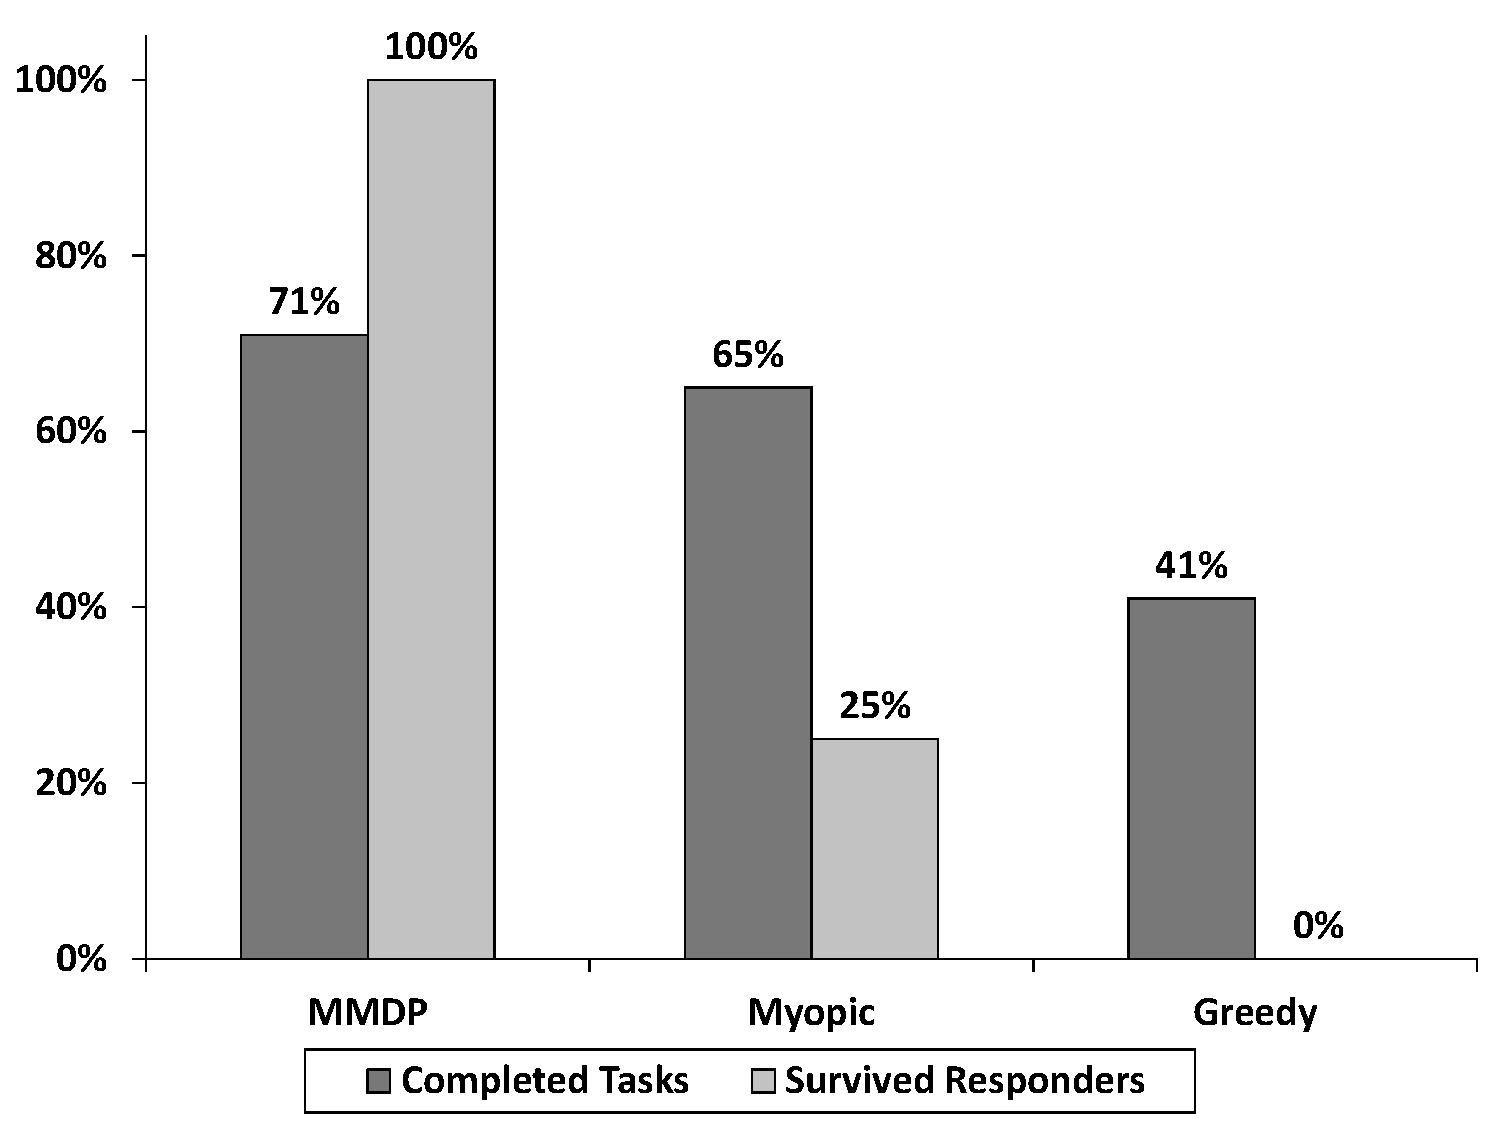
\includegraphics[width=0.8\linewidth]{simulation}
%  \caption{Experimental results for the MMDP, myopic, greedy
%  algorithms in simulation.}
%  \label{fig:simulation}
%\end{figure}


\noindent Before deploying our solution (as part of $PA$) to advise
human responders, it is important  to test its performance to
ensure it can return efficient solutions on simulations of the
real-world problem. Given there is no extant solution that
takes into account uncertainty in team coordination for emergency
response, we compare our algorithm with a greedy and a
myopic method to evaluate the benefits of coordination and
lookahead. For each method, we use our path planning algorithm to
compute the path for each responder. In the greedy method, the responders
are uncoordinated and select the closest tasks they can do. In
the myopic method, the responders are coordinated to select the
tasks but have no lookahead for the future tasks (Line 8 in
Algorithm~\ref{alg:taskplanning}). Table~\ref{tab:simulation} shows
the results for a problem with 17 tasks and 8 responders on a
50$\times$55 grid. As can be seen, our MMDP algorithm 
completes more tasks than the myopic and greedy methods (see Table
\ref{tab:simulation}). More importantly, our algorithm guarantees
the safety of the responders, while in the myopic method  only 25\%
of the responders survive and in the greedy method all responders
are killed by the radioactive cloud. More extensive evaluations are
beyond the scope of this paper as our focus here is on the use of
the algorithm in a field deployment to test how humans take up
advice computed by the planning agent $PA$.
\begin{table}[htbp]
  \centering
  \caption{Experimental results for the MMDP, myopic, greedy
  algorithms in simulation.}
  \begin{tabular}{l|c|c|c}
   & MMDP & Myopic & Greedy \\
  \hline
  No. of completed tasks & 71\% & 65\% & 41\% \\
  \hline
  No. responders alive at the end & 100\% & 25\% & 0\% \\
  \end{tabular}
  \label{tab:simulation}\vspace{-3mm}
\end{table}
